% 06.tex
% Benjamin Davies
% 2017 03 25

\begin{enumerate}

	\item
	Consider the constrained maximisation problem
	\[ \max_xf(x)=x(x^2-3)\ \text{s.t.}\ x\le1. 
		\label{eq:conmax1d_prob} \]
	%
	\begin{enumerate}

		\item
		Write down the Lagrangian for this problem.
		%
		\begin{solution}
			The Lagrangian is given by
			\[ \Lcal(x,\delta)=x(x^2-3)+\delta(1-x), \]
			where~$\delta$ is a Lagrange multiplier.
		\end{solution}

		\item
		Derive the first-order and complementary slackness conditions for an optimal solution to~\eqref{eq:conmax1d_prob}.
		%
		\begin{solution}
			The first-order condition for a maximum is
			%
			\begin{align}
				0
				&= \pder{\Lcal(x^*,\delta)}{x}\\
				&= 3(x^2-1)-\delta
			\end{align}
			%
			and the complementary slackness condition is
			\[ \delta(1-x^*)=0. \]
		\end{solution}

		\item
		Find the optimal solution~$x^*$ to~\eqref{eq:conmax1d_prob}.
		%
		\begin{solution}
			If~$\delta>0$ then~$x^*=1$ and if~$\delta=0$ then the first-order condition has roots~$x=\pm1$.
			Now~$f(1)=-2$ and~$f(-1)=2$, and so the optimal solution~$x^*=-1$.
		\end{solution}

	\end{enumerate}

	\item
	Consider the constrained maximisation problem
	\[ \max_xf(x)%
		=\ln(x_1x_2)\ \text{s.t.}\ %
			x_1+x_2\le1\ \text{and}\ x_1+2x_2\ge1. 
		\label{eq:conmax2d_prob} \]
	%
	\begin{enumerate}

		\item
		Write down the feasible set for this problem.
		Is this set convex?
		%
		\begin{solution}
			The feasible set is given by
			\[ X=\{x\in\R^2:x_1+x_2\le1\ \text{and}\ x_1+2x_2\ge1\}. \]
			This set is drawn below and is clearly convex.
			%
			\begin{center}
				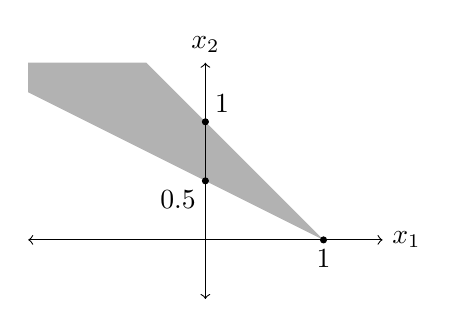
\begin{tikzpicture}[scale=1.5]

					% axes
					\draw [<->] (-1.5,0) -- (1.5,0) node [right] {$x_1$};
					\draw [<->] (0,-0.5) -- (0,1.5) node [above] {$x_2$};

					% set
					\fill [opacity=0.3] (-0.5,1.5) -- (1,0) -- (-1.5,1.25) -- (-1.5,1.5) -- cycle;

					% labels
					\draw [fill] (1,0) circle [radius=0.025] node [below] {$1$};
					\draw [fill] (0,0.5) circle [radius=0.025] node [below left] {$0.5$};
					\draw [fill] (0,1) circle [radius=0.025] node [above right] {$1$};

				\end{tikzpicture}
			\end{center}
		\end{solution}

		\item
		Write down the Lagrangian for this problem.
		%
		\begin{solution}
			The Lagrangian is given by
			\[ \Lcal(x,\delta)%
				=\ln(x_1x_2)+\delta_1(1-x_1-x_2)+\delta_2(x_1+2x_2-1), \]
			where~$\delta_1$ and~$\delta_2$ are Lagrange multipliers.
		\end{solution}

		\item
		Derive the first-order and complementary slackness conditions for an optimal solution to~\eqref{eq:conmax2d_prob}.
		%
		\begin{solution}
			The first-order conditions for a maximum are
			%
			\begin{align}
				0
				&= \pder{\Lcal(x^*,\delta)}{x_1}\\
				&= \frac{1}{x_1}-\delta_1+\delta_2\\
				0
				&= \pder{\Lcal(x^*,\delta)}{x_2}\\
				&= \frac{1}{x_2}-\delta_1+2\delta_2
			\end{align}
			%
			and the complementary slackness conditions are
			%
			\begin{align}
				\delta_1(1-x_1^*-x_2^*)
				&= 0\\
				\delta_2(x_1^*+2x_2^*-1)
				&= 0.
			\end{align}
		\end{solution}

		\item
		Find the optimal solution to~\eqref{eq:conmax2d_prob}.
		%
		\begin{solution}
			Suppose that~$\delta_1,\delta_2>0$.
			Then the complementary slackness conditions can be written as the linear system
			%
			\begin{align}
				x_1^*+x_2^*
				&= 1 \label{eq:conmax2d_csc1} \\
				x_1^*+2x_2^*
				&= 1
			\end{align}
			%
			which has unique solution~$x^*=(1,0)$.
			But the objective function is unbounded below as~$x^*\to0$, so this can't be a solution.
			Hence at most one constraint can bind.
			
			Suppose that~$\delta_1>0=\delta_2$.
			Then the first-order conditions imply that
			\[ x_1^*=x_2^*. \]
			Condition~\eqref{eq:conmax2d_csc1} then gives~$x_1^*=1/2$ and~$x_2^*=1/2$; a feasible solution.
			Hence the optimal solution~$x^*=(1/2,1/2)$.
		\end{solution}

	\end{enumerate}

	\item
	Consider the constrained \emph{minimisation} problem
	%
	\begin{align}
		\min_xf(x)=(x_1-1)^2+(x_2-2)^2\ \text{s.t.}\ x_1+x_2\le1.
			\label{eq:conmin_prob}
	\end{align}
	%
	\begin{enumerate}

		\item
		Write down the Lagrangian for this problem.
		%
		\begin{solution}
			The Lagrangian is given by
			\[ \mathcal{L}(x,\delta)
				=-(x_1-1)^2-(x_2-2)^2+\delta(1-x_1-x_2), \]
			where~$\delta$ is a Lagrange multiplier.
		\end{solution}

		\item
		Derive the first-order and complementary slackness conditions for an optimal solution to~\eqref{eq:conmin_prob}.
		%
		\begin{solution}
			The first-order conditions for a minimum are
			%
			\begin{align}
				\pder{\mathcal{L}(x^*,\delta)}{x_1}
				&= -2x_1^*+2-\delta\\
				&= 0 \label{eq:conmin_foc1}\\
				\pder{\mathcal{L}(x^*,\delta)}{x_2}
				&= -2x_2^*+4-\delta\\
				&= 0 \label{eq:conmin_foc2}
			\end{align}
			%
			and the complementary slackness condition is
			\[ \delta(1-x_1^*-x_2^*)=0. \]
		\end{solution}

		\item
		Find the optimal solution~$x^*$ to~\eqref{eq:conmin_prob}.
		%
		\begin{solution}
			Substituting~\eqref{eq:conmin_foc1} into~\eqref{eq:conmin_foc2} so as to eliminate~$\delta$ gives
			\[ 2-2x_1^*=4-2x_2^* \]
			so that
			\[ x_2^*=1+x_1^*. \]
			Hence
			%
			\begin{align}
				1
				&\ge x_1^*+x_2^*\\
				&= 1+2x_1^*
			\end{align}
			%
			and therefore
			\[ x_1^*\le0. \]
			If~$x_1^*<0$ then~$x_2^*<1$ and the complementary slackness condition implies that~$\delta=0$.
			But then~\eqref{eq:conmin_foc1} gives~$x_1^*=1\not<0$, a contradiction.
			Hence we must have~$x_1^*=0$.
			This gives~$x_2^*=1$ and~$\delta=2$, which is feasible.
			It follows that the optimal solution~$x^*=(0,1)$.
		\end{solution}

		\item
		Interpret the Lagrange multiplier for the contraint~$x_1+x_2\le1$.
		%
		\begin{solution}
			We know that~$\delta=2$ from part~c).
			The constraint is binding on the optimal solution because~$\delta>0$.
			If we relaxed this constraint then we would expect the optimal objective function value to \emph{decrease}.
		\end{solution}

	\end{enumerate}

\end{enumerate}
